\documentclass[10pt]{article}

\usepackage{anysize} % Package to change margin size
	\marginsize{2cm}{2cm}{1cm}{2cm}

\usepackage{fancyhdr} % Package to make headers
	\renewcommand{\headrulewidth}{0pt}

\usepackage[dvipsnames]{xcolor} % Colors for the references links

\usepackage{hyperref} % Package to link references
	\hypersetup{colorlinks=true, linkcolor=black, citecolor=CadetBlue, filecolor=CadetBlue, urlcolor=CadetBlue,
}

\usepackage{multicol} % Package for multicolumn

\usepackage{float} % Figures in multicolumn

\usepackage[justification=centering]{caption} % Caption package

\usepackage{parskip} % Package for removing paragraph indentations
	\setlength\columnsep{18pt}

\usepackage{amsmath, amssymb, amsfonts, mathtools, gensymb} % Package for maths

\usepackage{enumerate} % Package for numeration list

\usepackage{textcomp} % Euro sign

\usepackage[style=numeric,
			backend=bibtex]{biblatex} % Package for references
\addbibresource{references.bib}
	
\usepackage{graphicx} \graphicspath{ {./images/} }

\usepackage{multirow} % Package for multiple rows

%\newcommand{\squeezeup}{\vspace{-2.5mm}}

\usepackage{etoolbox}

\BeforeBeginEnvironment{figure}{\vskip-1ex}
\AfterEndEnvironment{figure}{\vskip-1ex}

\usepackage{titlesec} % Adjust section spacing
\titlespacing\section{0pt}{0pt plus 4pt minus 2pt}{0pt plus 2pt minus 2pt}
\titlespacing\subsection{0pt}{12pt plus 4pt minus 2pt}{0pt plus 2pt minus 2pt}

\setlength{\textfloatsep}{10pt plus 1.0pt minus 2.0pt}

\begin{document}

% Makes header	
\pagestyle{fancy}
\fancyhead[R]{\textit{EE4513}}% - Paper}}
\fancyhead[L]{\textit{Seminar Paper}}

% Makes footnotes with an asterisk NOT NECESSARY

% Title
\begin{center}
	\Large{\textbf{Why is Germany experiencing an EV boom despite economic challenges?}}
	\normalsize

	% Author
	\textit{Patryk Eryk Merino-Wi{\'s}niewski}\\
	\vspace{0.1cm}
	%Additional information
	\textit{A0293826R}
	\medskip
	\normalsize
\end{center}

\begin{multicols}{2}
	\small\textit{This paper was supported in part by the use of ChatGPT, an AI language model developed by OpenAI. The tool was used to enhance phrasing, check grammar, and assist in providing vehicle-related data.
	}\normalsize 
	\section{Introduction} \label{sec: intro}
		In recent years, Germany has witnessed a remarkable surge in the adoption of electric vehicles (EVs), positioning itself as one of the leading EV markets in Europe. This rapid growth is especially striking given the country’s broader economic headwinds, including slowing GDP growth, inflationary pressures, and supply chain disruptions. Traditionally known for its powerful combustion engine legacy and deep-rooted automotive culture, Germany's pivot toward electromobility signals a significant transformation not only in consumer preferences but also in industrial strategy and environmental policy.

Understanding the factors driving this EV boom requires a closer look at the interplay between government incentives, regulatory pressures, evolving consumer behavior, and the strategic responses of German automakers. This paper seeks to explore the underlying reasons why Germany, despite facing economic challenges, is experiencing such a strong shift toward electric mobility. By doing so, it sheds light on the broader implications for the automotive industry, energy infrastructure, and the country’s climate ambitions.

	\section{EV Market}\label{sec: mark}
		\begin{figure}[H]
	\begin{center}
		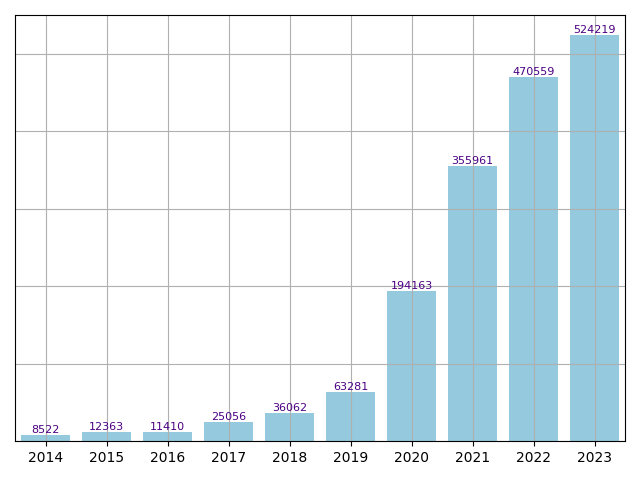
\includegraphics[width=\linewidth]{images/EV_amount.png}
	\end{center}
	\caption{Amount of new EVs on Road}
	\label{fig: ev_market}
	\captionsetup{font={footnotesize,bf,it}}
  	\caption*{Data: European Commission, \cite{Estat}} 
\end{figure}
Figure \ref{fig: ev_market} illustrates the number of newly purchased EVs in the market from 2014 to 2023. The most remarkable change, or rather 'boom', occurred in 2020. The most remarkable change, arguably a true boom, occurred in 2020. Coincidentally, 2020 was also the year of the COVID-19 outbreak. Germany has undergone astonishing changes over the past five years, but so far, we have only looked at EV-specific figures. To better understand the scale of this shift, let’s now consider the total number of newly registered vehicles overall.
\begin{figure}[H]
	\begin{center}
		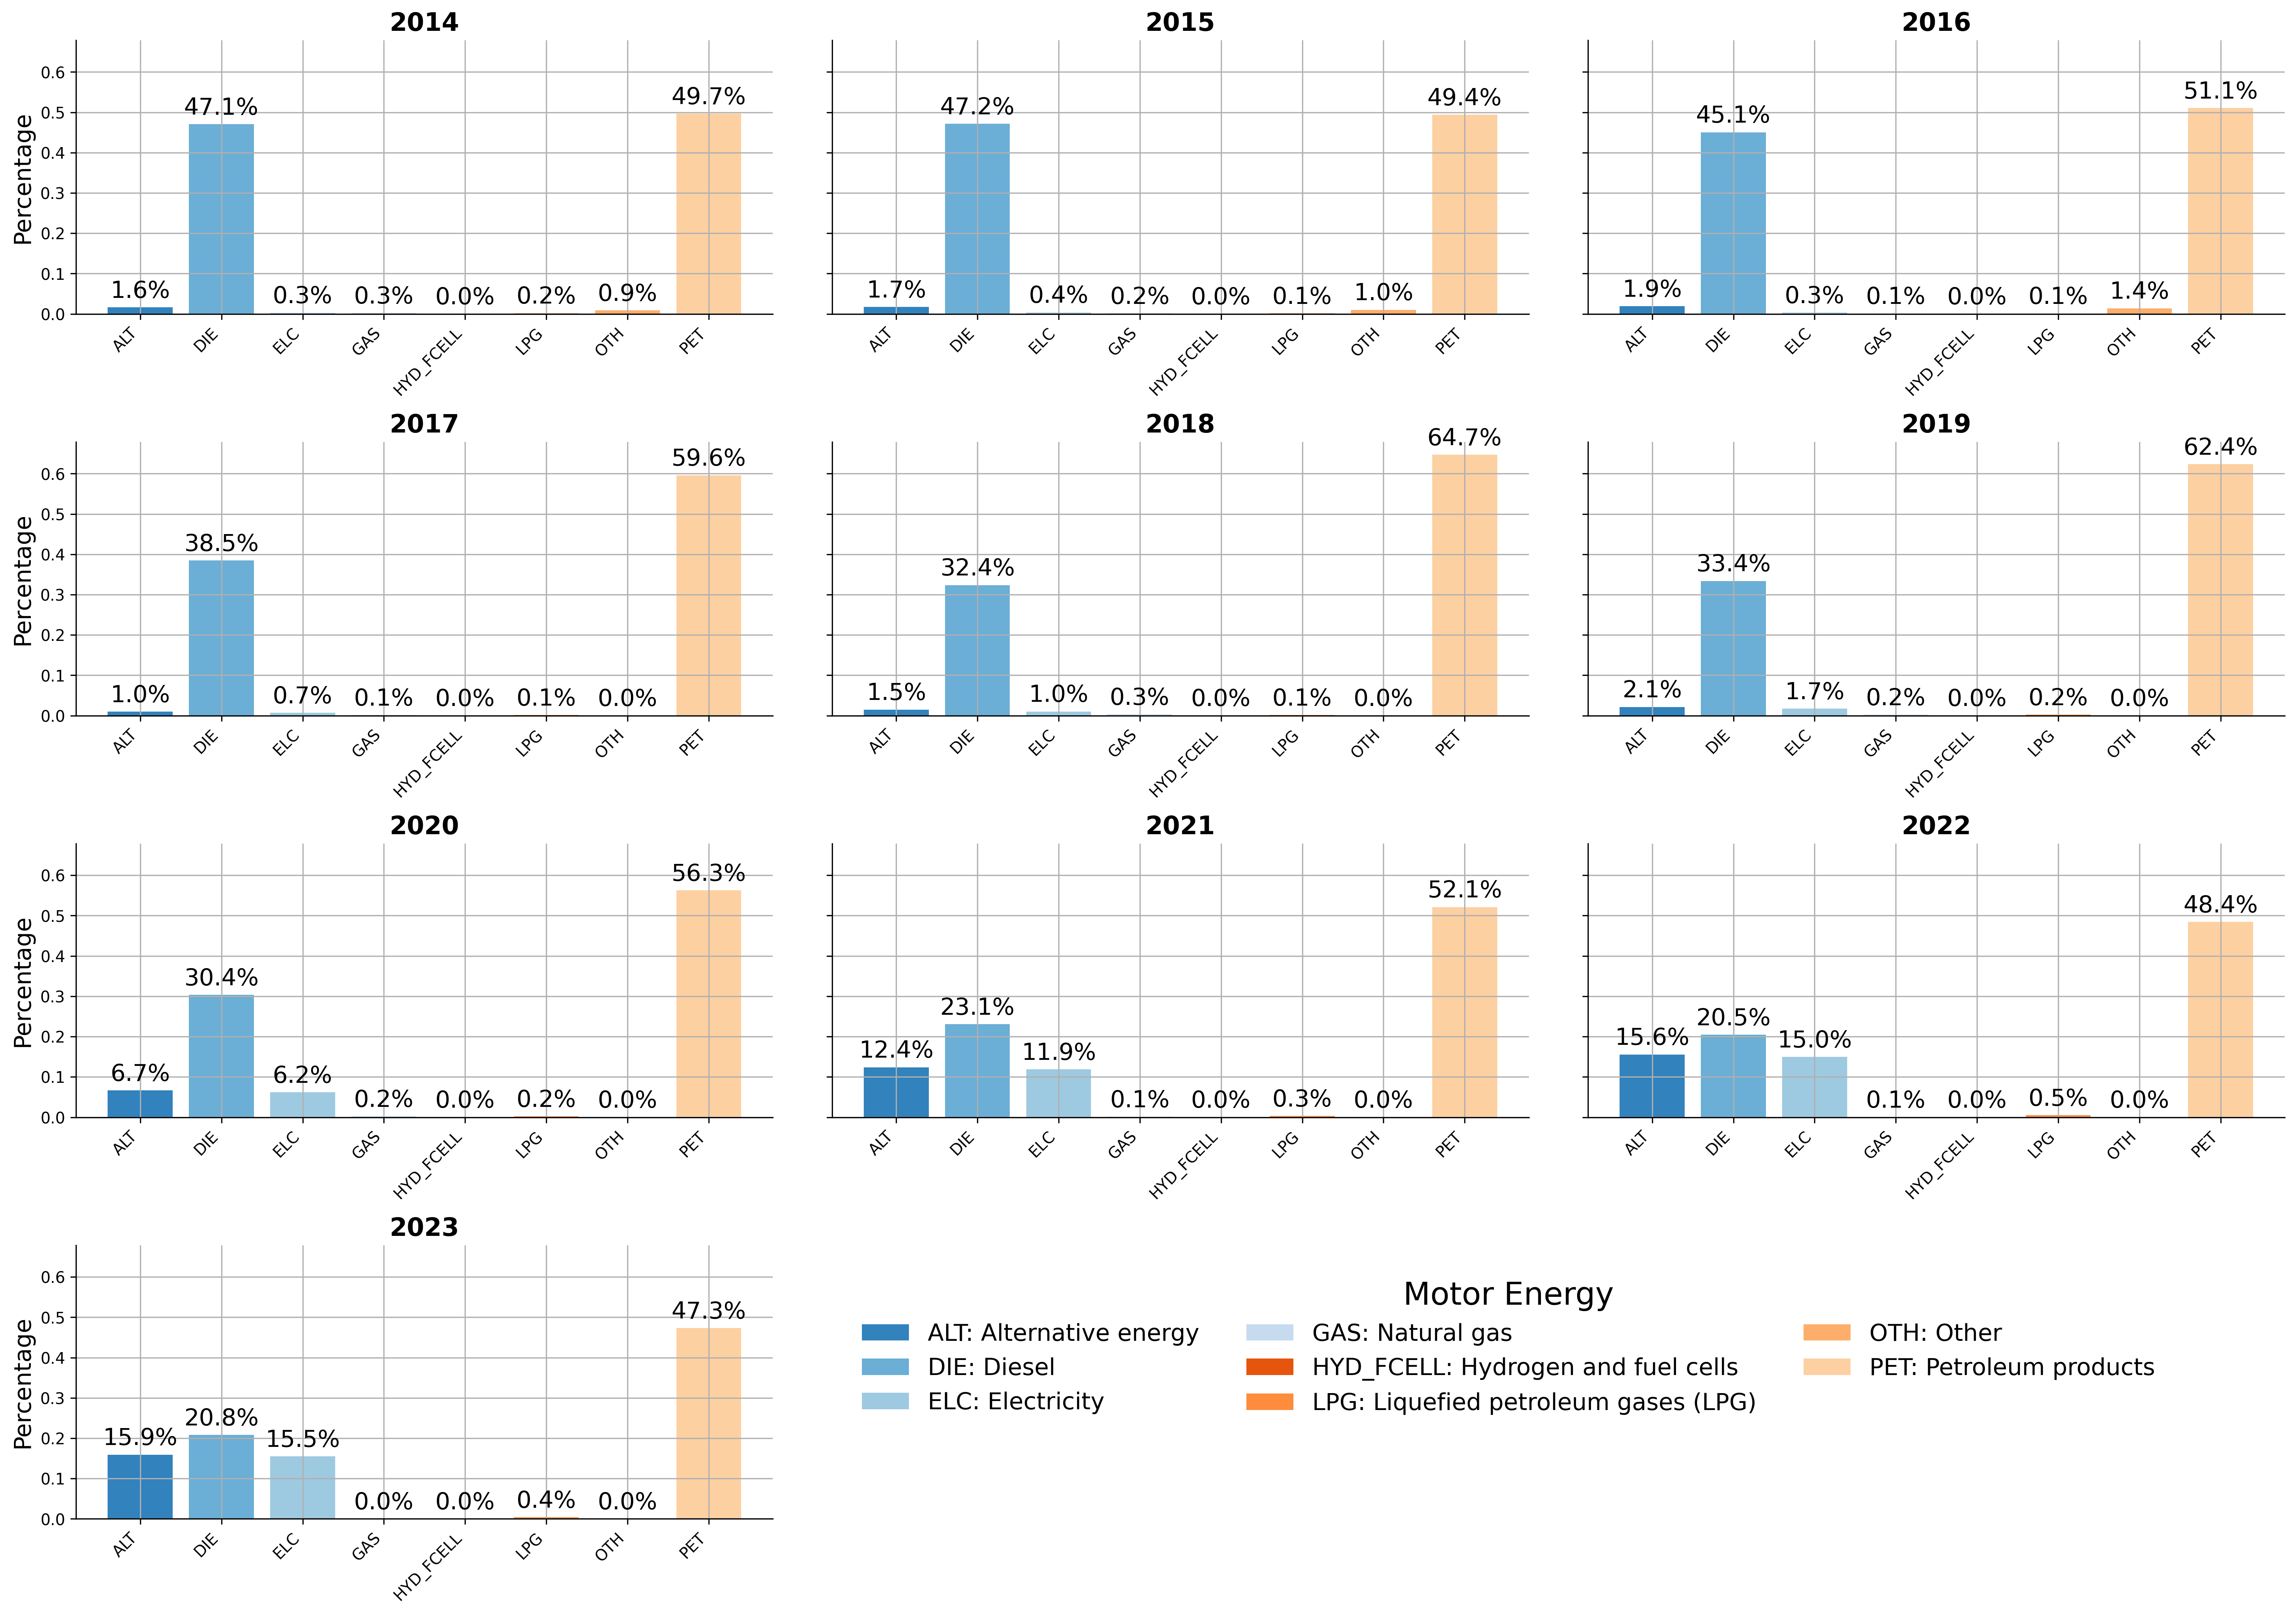
\includegraphics[width=\linewidth]{images/Veh_Mark.png}
		\caption{Percentage Distribution of Motor Energy Types in Vehicles Over Time}
		\label{fig: vehicles_market}
		\captionsetup{font={footnotesize,bf,it}}
  		\caption*{Data: European Commission, \cite{Estat}}
	\end{center}
\end{figure}
The development of electric mobility has been on a rise since 2016, s. Fig. \ref{fig: vehicles_market}. It is important to note that the data excludes hybrid vehicles as their primary energy source remains fossil fuels. The most notable shift in the yearly share of newly registered electric vehicles occurred in 2020, with an increase of 5.7 percentage points. Another indicator of progress toward sustainable energy in the transport sector is the decline in both diesel and petrol vehicle registrations, accompanied by a steady rise in alternative powertrains. 

Another valuable dataset concerns the distribution of EVs between districts, s. Fig. \ref{fig: districts}. The disparity in EV ownership is evident when comparing East Germany—formerly the German Democratic Republic (GDR) under Soviet influence prior to reunification—with West Germany, which emerged as a prosperous free-market state after World War II. To this day, differences across various socio-economic categories between East and West Germany persist. A more detailed discussion on this topic can be found in \cite{BundestagOstWest}.
\begin{figure}[H]
	\begin{center}
		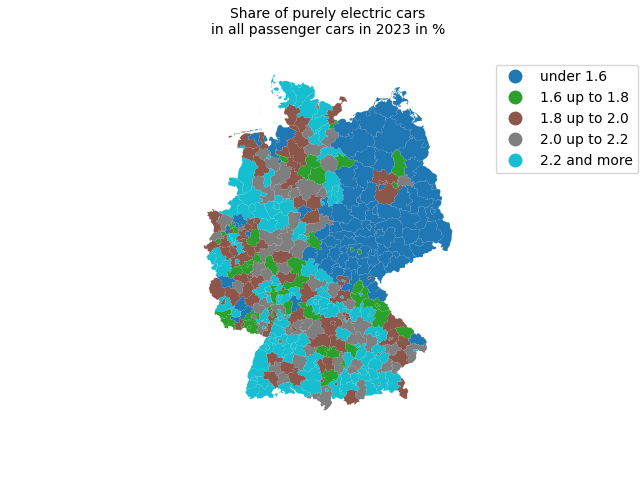
\includegraphics[width=\linewidth]{images/EV_percentage.png}
		\caption{Distribution of Electric Vehicles Across German Districts}
		\label{fig: districts}
		\captionsetup{font={footnotesize,bf,it}}
  		\caption*{Data: Deutschlandatlas, \cite{DeAtlasEVXLSX} \\
  				Map: BKG, \cite{BKG} } 
  	\end{center}
\end{figure}
The calculations below highlight the differences in EV ownership between densely populated urban areas and rural districts, s. Fig. \ref{fig: ev_percentage}. The values are based on the mean EV share within each category to ensure a representative comparison.
\begin{figure}[H]
	\begin{center}
		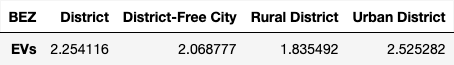
\includegraphics[width=\linewidth]{images/EVs_mean.png}
		\caption{Geographic Distribution of EV Ownership}
		\label{fig: ev_percentage}
		%\captionsetup{font={footnotesize,bf,it}}
  		%\caption*{Data: Deutschlandatlas, \cite{DeAtlasEVXLSX}}
	\end{center}
\end{figure}
Rural districts tend to have fewer electric vehicles compared to urban areas and cities, which could be attributed to limited charging infrastructure.
	

	\section{Charging Infrastructure}\label{sec: charg}
		An important factor when deciding whether to purchase any type of vehicle is access to the corresponding fuel source. However, this consideration tends to be less critical for conventional vehicles, as their significantly greater range compared to EVs reduces dependency on frequent refueling infrastructure. Figure \ref{fig: charg_stat} demonstrates the number of charging stations per 100,000 inhabitants.

As of October 1st, 2023, there are approximately 108,000 public charging points across Germany, including around 21,000 fast charging stations. The previous government coalition had set an ambitious goal of expanding the charging infrastructure to one million stations by 2030. Once again, the most densely covered regions are found in the South—particularly in Bavaria and Baden-Württemberg, while the eastern states continue to lag behind in comparison to the West \cite{DeAtlasCharge}.
\begin{figure}[H]
	\begin{center}
		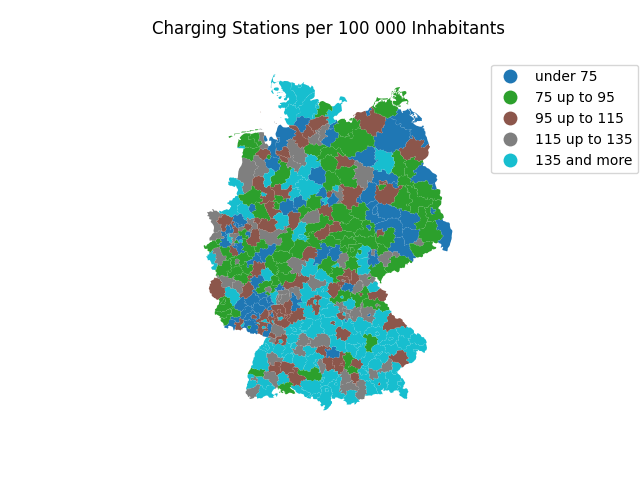
\includegraphics[width=\linewidth]{images/Charging_stations}
		\caption{Distribution of Charging Station Across German District}
		\label{fig: charg_stat}
		\captionsetup{font={footnotesize,bf,it}}
		\caption*{Data: Deutschlandatlas, \cite{DeAtlasEVXLSX} \\
  				Map: BKG, \cite{BKG} } 
	\end{center} 
\end{figure}
The calculated means of charging stations across different administrative categories (see Fig. \ref{fig: mean_charg}) show that urban districts have greater access to charging infrastructure. The 
\begin{figure}[H]
	\begin{center}
		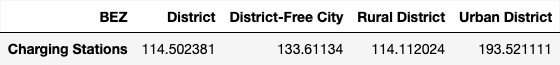
\includegraphics[width=\linewidth]{images/Charg_mean.png}
	\end{center}
	\caption{Distribution of Charging Stations}
	\label{fig: mean_charg}
\end{figure}
The calculated means of charging stations across different administrative groups show that urban districts have significantly greater access to charging infrastructure, s. Fig. \ref{fig: mean_charg}. This disparity likely reflects differences in population density, investment priorities, and the broader push for urban sustainability

	\section{Energy Price Comparison}\label{sec: ener}
		Fuel prices significantly influence transportation choices, affecting both consumer behavior and industry trends. While the cost of traditional fuels like petroleum and diesel remains a key factor, the growing shift to electric vehicles (EVs) brings electricity prices into focus. This section examines the pricing dynamics of electricity and fossil fuels, shedding light on the economic factors that impact their costs.

Figure \ref{fig: fuel_prices} illustrates the price changes over the past 20 years. Both fuel types follow similar trends, with diesel typically being cheaper than its counterpart. As of April 7th, 2025, the prices for petroleum and diesel were \texteuro 1,785 and \texteuro1,551 per 1,000 liters, respectively.

\begin{figure}[H]
	\begin{center}
		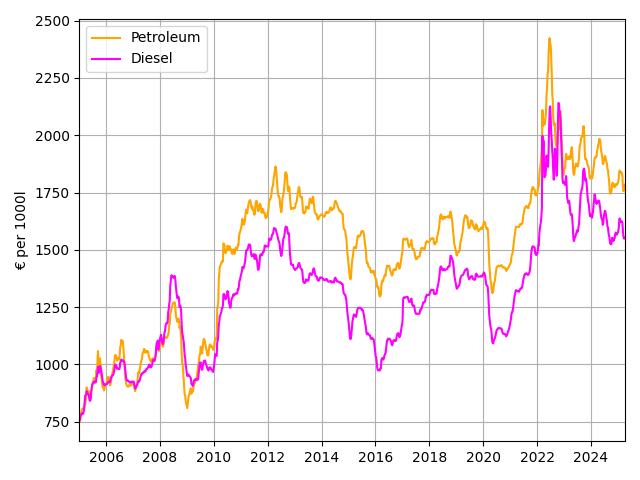
\includegraphics[width=\linewidth]{images/gas_diesel_prices.png}
		\caption{Fuel Prices throughout the Years}
		\label{fig: fuel_prices}
		\captionsetup{font={footnotesize,bf,it}}
		\caption*{Data: European Commission, \cite{PriceDevelopments}} 
	\end{center}
\end{figure}
Figure \ref{fig: electr_bill} shows the electricity bill values for consumers, divided into two categories: households and non-households. Non-household consumers, such as charging point operators and industrial users, often benefit from more favorable rates due to higher efficiency, larger volumes, and more consistent demand. The specific types of distributors are listed in the legend of Figure \ref{fig: electr_bill}. A noticeable peak in household electricity expenses occurred following the onset of the Ukraine-Russia war. For non-households, prices have shown a general upward trend over time. In 2023, the Preisbremse (price cap) was introduced to mitigate the economic impact of the energy crisis. \cite{BundesregierungStromPreisBremse}
\begin{figure}[H]
	\begin{center}
		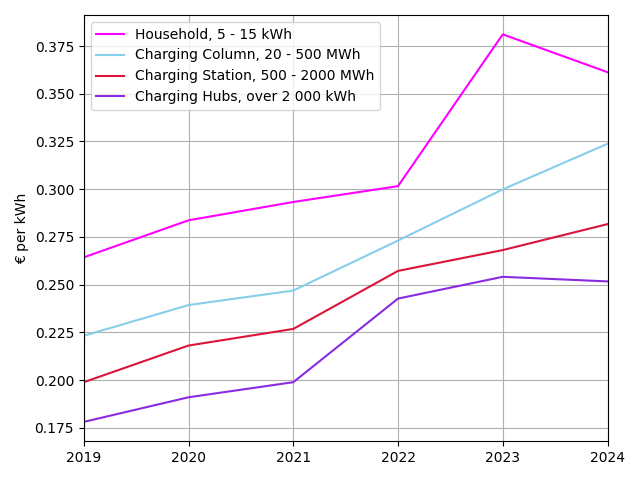
\includegraphics[width=\linewidth]{images/Elec_price.png}
	\caption{Charging Cost per kWh over the Years}
	\label{fig: electr_bill}
	\captionsetup{font={footnotesize,bf,it}}
	\caption*{Data: Statistisches Bundesamt, \cite{DestatisStrompreise}, \cite{GENESISHaushalt}, \cite{GENESISNichtHaushalt}}
	\end{center}
\end{figure}

It is important to note that the electricity bill values presented do not reflect the actual prices consumers pay when charging their electric vehicles (EVs), but rather the average electricity prices paid by households and non-household distributors for grid energy. Home charging is classified as slow charging, while a column typically refers to slow or normal public charging. A station provides fast charging, and a hub is used for ultra-fast charging, offering the quickest recharge times. Since detailed pricing data for individual distributor types was unavailable, representative values were estimated using ChatGPT: \texteuro0.49 for standard columns, \texteuro0.59 for stations, \texteuro0.69 for hubs, and \texteuro0.40 for Tesla Superchargers. A grid efficiency factor of 85\% was also applied to account for typical charging losses. Additionally, ChatGPT provided estimated vehicle data—such as tank size, battery capacity, and electric (RE) and combustion (RC) ranges by body type—which is summarized in Figure \ref{fig: vehic_data} to support the simplified cost model.
\begin{figure}[H]
	\begin{center}
		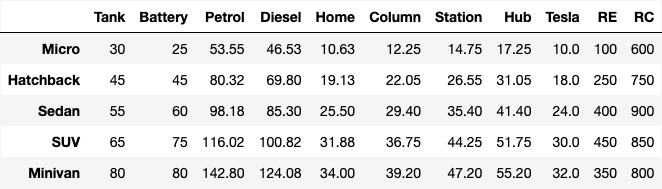
\includegraphics[width=\linewidth]{images/Prices_summary.png}
		\caption{Representative Fuel and Range Data for Cost Modeling}
		\label{fig: vehic_data}
		\captionsetup{font={footnotesize,bf,it}}
		\caption*{Data: ChatGPT (Estimates)}
	\end{center}	
\end{figure}
To assess the cost-efficiency of different vehicle types, a simplified metric was used by dividing the estimated driving range by the corresponding fuel or electricity price. This results in a “distance per euro” value, which reflects how many kilometers a vehicle can travel per unit of currency spent on energy.  While not a conventional efficiency measure like energy consumption per kilometer, it provides a useful comparison of economic driving performance across vehicle types and energy sources. This cost-based driving efficiency highlights the financial advantage of electric vehicles in scenarios with lower electricity prices and high energy efficiency
\begin{figure}[H]
	\begin{center}
		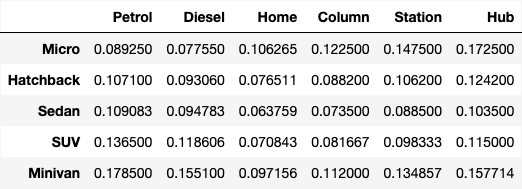
\includegraphics[width=\linewidth]{images/cost_efficiency.png}
		\caption{Cost Efficiency}
		\label{fig: Driving Efficiency}
		\captionsetup{font={footnotesize,bf,it}}
		\caption*{Data: ChatGPT (Estimates)}
	\end{center}	
\end{figure}
The cost per kilometer is consistently lower for electric vehicles compared to petrol and diesel across non-micro body types, especially when charged at home. Larger vehicles like SUVs and minivans show a more significant cost advantage when using home or standard charging options, highlighting the economic benefit of EVs in higher consumption segments. This analysis has focused on one aspect of a car's cost—charging expenses. However, a complete evaluation of a vehicle’s total cost of ownership also includes factors like resale value and operational costs.

	\section{The Economics of EV Ownership}\label{sec: owner}
		Resale values for electric vehicles (EVs) are generally lower than for traditional petrol and diesel cars, primarily due to faster depreciation rates. Despite this, operational costs for EVs tend to be significantly lower, as they require less maintenance and the cost of electricity is usually cheaper than fuel.

A recent study examining EV pricing in Germany between 2015 and 2020 found that luxury and mid-sized EVs are expected to reach purchase price parity with conventional vehicles by 2023 and 2026, respectively, while small EVs may not do so before 2030. The total cost of ownership for larger EVs was already comparable to combustion vehicles by 2020, even without subsidies. However, small EVs still depend heavily on financial support, underlining the need for further innovation and policy incentives. \cite{goetzel2022empirical}

The internal combustion engine (ICE) systems in EREVs are less costly than in conventional ICE vehicles due to simpler transmission design. Electric motor costs are also declining steadily with increased production volumes. For EVs, additional expenses such as potential battery replacements—estimated based on load cycles—must be considered. While HEVs and FCHEVs generally avoid this due to limited battery use, BEVs and EREVs may require replacements over their lifetime. Other ongoing costs include maintenance, insurance, and vehicle taxes. A detailed total cost of ownership analysis in Germany, covering six vehicle classes, three user types, and various drive technologies for 2015, 2030, and 2050, found that only mild and full hybrids are economically viable without subsidies, primarily for high-mileage users. In contrast, fully electric and extended-range vehicles remain financially unfeasible without government support, despite policy focus on their adoption. \cite{owid-co2-emissions-from-transport}
		
	\section{Government Policies and Incentives}\label{sec: gover}
		Road travel is responsible for three-quarters of transport emissions, with passenger vehicles (cars and buses) contributing 45.1\%, and trucks carrying freight accounting for 29.4\%. \cite{owid-co2-emissions-from-transport}

The European Union's decision to prohibit the sale of new petrol and diesel cars from 2035 have accelerated governments to act promptly to achieving climate neutrality by 2050. \cite{TopicsEuParliament}

As mentioned in Section \ref{sec: charg}, the development of charging stations is a key measure to achieve climate neutrality by 2050. The previous government aimed for 15 million fully electric passenger cars by 2030, a challenging goal. The current government under Chancellor Merz has introduced an 8-step plan for EVs, including:
\begin{enumerate}
	\item Increasing the tax incentive limit for company cars to €100,000 (up from €70,000) \cite{FrankfurterRundschau}.
	\item A special depreciation allowance for electric vehicles.
	\item Vehicle tax exemption for EVs until 2035 \cite{BusinessInsider}.
	%\item Support for low- and medium-income households transitioning to climate-friendly mobility, funded by the EU Climate Social Fund.
	%\item Promotion of plug-in hybrids (PHEVs) and electric vehicles with range extenders (EREVs) and corresponding European regulations.
	%\item Acceleration of charging network expansion, including fast-charging stations and commercial depot charging.
	%\item Toll exemptions for zero-emission trucks after 2026.
	%\item Promotion of hydrogen infrastructure for commercial vehicles \cite{BusinessInsider}.
\end{enumerate}
To accelerate the adoption of electric vehicles, a range of incentives can be implemented. These include monetary incentives such as purchase premiums, scrappage bonuses, subsidized loans, special depreciation schemes for commercial EVs, and tax benefits. Non-monetary incentives involve measures like reserved parking spots, access to bus lanes, dedicated EV lanes or charging zones, low-emission zones, and congestion charges based on pollution levels. \cite{owid-co2-emissions-from-transport}

	\section{Conclusion}\label{sec: conc}
		Germany’s current EV boom, unfolding in the midst of economic uncertainty, is the outcome of a complex yet well-directed policy and market evolution. The steadily increasing number of EVs on the road reflects both consumer confidence in the technology and strong political will to decarbonize the transport sector. Key drivers include rising fuel prices, growing environmental consciousness, and a broad range of government-led incentives, from tax breaks to direct purchase subsidies.

However, for the transition to be sustainable and equitable, existing gaps must be addressed. The discrepancy in charging infrastructure between East and West Germany, as well as between urban and rural regions, poses a significant challenge to widespread adoption. To ensure that all citizens benefit from the mobility shift, a more balanced and inclusive rollout of charging networks is necessary.

Additionally, stabilizing electricity prices should be a priority. As charging costs become a growing concern for both private and commercial EV users, protecting consumers from further price surges is essential to maintain EV affordability. Alongside this, Germany must continue to invest in research and innovation to enhance battery technologies, charging efficiency, and overall vehicle performance.

Finally, further reductions in EV-related taxes and insurance premiums, combined with expanded subsidy programs, will be crucial for improving the total cost of ownership—particularly for lower- and middle-income households. These coordinated efforts can help transform the current momentum into a resilient and long-term shift, solidifying Germany’s position as a leader in clean and future-ready mobility.
		
	\section*{References}


\printbibliography[type=article, title={Articles}]

\printbibliography[type=online, title={Online Resources}]

\clearpage
\end{multicols}

\end{document}
	
\end{document}